%%%%%%%%%%%%%%%%%%%%%%%%%%%%%%%%%%%%%%%%%
% Lachaise Assignment
% LaTeX Template
% Version 1.0 (26/6/2018)
%
% This template originates from:
% http://www.LaTeXTemplates.com
%
% Authors:
% Marion Lachaise & François Févotte
% Vel (vel@LaTeXTemplates.com)
%
% License:
% CC BY-NC-SA 3.0 (http://creativecommons.org/licenses/by-nc-sa/3.0/)
% 
%%%%%%%%%%%%%%%%%%%%%%%%%%%%%%%%%%%%%%%%%

%----------------------------------------------------------------------------------------
%	PACKAGES AND OTHER DOCUMENT CONFIGURATIONS
%----------------------------------------------------------------------------------------

\documentclass{article}
\usepackage{float}
\usepackage{fancyvrb}

%%%%%%%%%%%%%%%%%%%%%%%%%%%%%%%%%%%%%%%%%
% Lachaise Assignment
% Structure Specification File
% Version 1.0 (26/6/2018)
%
% This template originates from:
% http://www.LaTeXTemplates.com
%
% Authors:
% Marion Lachaise & François Févotte
% Vel (vel@LaTeXTemplates.com)
%
% License:
% CC BY-NC-SA 3.0 (http://creativecommons.org/licenses/by-nc-sa/3.0/)
% 
%%%%%%%%%%%%%%%%%%%%%%%%%%%%%%%%%%%%%%%%%

%----------------------------------------------------------------------------------------
%	PACKAGES AND OTHER DOCUMENT CONFIGURATIONS
%----------------------------------------------------------------------------------------

\usepackage{amsmath,amsfonts,stmaryrd,amssymb} % Math packages

\usepackage{enumerate} % Custom item numbers for enumerations

\usepackage[ruled]{algorithm2e} % Algorithms

\usepackage[framemethod=tikz]{mdframed} % Allows defining custom boxed/framed environments

\usepackage{listings} % File listings, with syntax highlighting
\lstset{
	basicstyle=\ttfamily, % Typeset listings in monospace font
}

%----------------------------------------------------------------------------------------
%	DOCUMENT MARGINS
%----------------------------------------------------------------------------------------

\usepackage{geometry} % Required for adjusting page dimensions and margins

\geometry{
	paper=a4paper, % Paper size, change to letterpaper for US letter size
	top=2.5cm, % Top margin
	bottom=3cm, % Bottom margin
	left=2.5cm, % Left margin
	right=2.5cm, % Right margin
	headheight=14pt, % Header height
	footskip=1.5cm, % Space from the bottom margin to the baseline of the footer
	headsep=1.2cm, % Space from the top margin to the baseline of the header
	%showframe, % Uncomment to show how the type block is set on the page
}

%----------------------------------------------------------------------------------------
%	FONTS
%----------------------------------------------------------------------------------------

\usepackage[utf8]{inputenc} % Required for inputting international characters
\usepackage[T1]{fontenc} % Output font encoding for international characters

\usepackage{XCharter} % Use the XCharter fonts

%----------------------------------------------------------------------------------------
%	COMMAND LINE ENVIRONMENT
%----------------------------------------------------------------------------------------

% Usage:
% \begin{commandline}
%	\begin{verbatim}
%		$ ls
%		
%		Applications	Desktop	...
%	\end{verbatim}
% \end{commandline}

\mdfdefinestyle{commandline}{
	leftmargin=10pt,
	rightmargin=10pt,
	innerleftmargin=15pt,
	middlelinecolor=black!50!white,
	middlelinewidth=2pt,
	frametitlerule=false,
	backgroundcolor=black!5!white,
	frametitle={Output},
	frametitlefont={\normalfont\sffamily\color{white}\hspace{-1em}},
	frametitlebackgroundcolor=black!50!white,
	nobreak,
}

% Define a custom environment for command-line snapshots
\newenvironment{commandline}{
	\medskip
	\begin{mdframed}[style=commandline]
}{
	\end{mdframed}
	\medskip
}

%----------------------------------------------------------------------------------------
%	FILE CONTENTS ENVIRONMENT
%----------------------------------------------------------------------------------------

% Usage:
% \begin{file}[optional filename, defaults to "File"]
%	File contents, for example, with a listings environment
% \end{file}

\mdfdefinestyle{file}{
	innertopmargin=1.6\baselineskip,
	innerbottommargin=0.8\baselineskip,
	topline=false, bottomline=false,
	leftline=false, rightline=false,
	leftmargin=2cm,
	rightmargin=2cm,
	singleextra={%
		\draw[fill=black!10!white](P)++(0,-1.2em)rectangle(P-|O);
		\node[anchor=north west]
		at(P-|O){\ttfamily\mdfilename};
		%
		\def\l{3em}
		\draw(O-|P)++(-\l,0)--++(\l,\l)--(P)--(P-|O)--(O)--cycle;
		\draw(O-|P)++(-\l,0)--++(0,\l)--++(\l,0);
	},
	nobreak,
}

% Define a custom environment for file contents
\newenvironment{file}[1][File]{ % Set the default filename to "File"
	\medskip
	\newcommand{\mdfilename}{#1}
	\begin{mdframed}[style=file]
}{
	\end{mdframed}
	\medskip
}

%----------------------------------------------------------------------------------------
%	NUMBERED QUESTIONS ENVIRONMENT
%----------------------------------------------------------------------------------------

% Usage:
% \begin{question}[optional title]
%	Question contents
% \end{question}

\mdfdefinestyle{question}{
	innertopmargin=1.2\baselineskip,
	innerbottommargin=0.8\baselineskip,
	roundcorner=5pt,
	nobreak,
	singleextra={%
		\draw(P-|O)node[xshift=1em,anchor=west,fill=white,draw,rounded corners=5pt]{%
		Question \theQuestion\questionTitle};
	},
}

\newcounter{Question} % Stores the current question number that gets iterated with each new question

% Define a custom environment for numbered questions
\newenvironment{question}[1][\unskip]{
	\bigskip
	\stepcounter{Question}
	\newcommand{\questionTitle}{~#1}
	\begin{mdframed}[style=question]
}{
	\end{mdframed}
	\medskip
}

%----------------------------------------------------------------------------------------
%	WARNING TEXT ENVIRONMENT
%----------------------------------------------------------------------------------------

% Usage:
% \begin{warn}[optional title, defaults to "Warning:"]
%	Contents
% \end{warn}

\mdfdefinestyle{warning}{
	topline=false, bottomline=false,
	leftline=false, rightline=false,
	nobreak,
	singleextra={%
		\draw(P-|O)++(-0.5em,0)node(tmp1){};
		\draw(P-|O)++(0.5em,0)node(tmp2){};
		\fill[black,rotate around={45:(P-|O)}](tmp1)rectangle(tmp2);
		\node at(P-|O){\color{white}\scriptsize\bf !};
		\draw[very thick](P-|O)++(0,-1em)--(O);%--(O-|P);
	}
}

% Define a custom environment for warning text
\newenvironment{warn}[1][Warning:]{ % Set the default warning to "Warning:"
	\medskip
	\begin{mdframed}[style=warning]
		\noindent{\textbf{#1}}
}{
	\end{mdframed}
}

%----------------------------------------------------------------------------------------
%	INFORMATION ENVIRONMENT
%----------------------------------------------------------------------------------------

% Usage:
% \begin{info}[optional title, defaults to "Info:"]
% 	contents
% 	\end{info}

\mdfdefinestyle{info}{%
	topline=false, bottomline=false,
	leftline=false, rightline=false,
	nobreak,
	singleextra={%
		\fill[black](P-|O)circle[radius=0.4em];
		\node at(P-|O){\color{white}\scriptsize\bf i};
		\draw[very thick](P-|O)++(0,-0.8em)--(O);%--(O-|P);
	}
}

% Define a custom environment for information
\newenvironment{info}[1][Info:]{ % Set the default title to "Info:"
	\medskip
	\begin{mdframed}[style=info]
		\noindent{\textbf{#1}}
}{
	\end{mdframed}
}
 % Include the file specifying the document structure and custom commands

%----------------------------------------------------------------------------------------
%	ASSIGNMENT INFORMATION
%----------------------------------------------------------------------------------------


%----------------------------------------------------------------------------------------

\begin{document}


\begin{titlepage}
    \begin{center}
        \vspace*{5cm}
 
        \Huge
        \textbf{Data Mining Final Project}
 
        \vspace{0.5cm}
        \LARGE
        Suicide Attempt Prediction using Classification
 
        \vspace{1.5cm}
 
        \textbf{Arif Ahmet Balik}\\
        180303019
 
        \vfill
 
 
        \vspace{0.8cm}
 
        %\includegraphics[width=0.4\textwidth]{university}
 
        \Large
        Computer Engineering\\
        Istanbul Arel University\\
        Buyukcekmece, Turkey\\
        21.05.2019
 
    \end{center}
\end{titlepage}
%----------------------------------------------------------------------------------------
%	INTRODUCTION
%----------------------------------------------------------------------------------------

\section*{Introduction} % Unnumbered section

This report covers prediction and analysis of \textit{ForeverAlone} dataset which will be described in Data section. The aim is to create a model that can accurately predict suicidal status of a person based on some of their personal data. Throughout the modeling, a few different method will be tested (Decision tree, rainforest, etc.). There will be experiments on different settings of data modeling experiments, and results will be discussed in more detail. Also data normalization, and reasoning on the dataset will be shown in steps.

At the end a model will be chosen and source code will be added in the document. 


%----------------------------------------------------------------------------------------
%	PROBLEM 1
%----------------------------------------------------------------------------------------

\section{Dataset and Normalization} % Numbered section

The dataset is created with contributions of reddit users on the subreddit \textit{ /r/ForeverAlone}. A first look at data columns gives a hint for which features can be used to create a stable model.

\begin{figure}[H]
\centering
\begin{BVerbatim}
time [date]
gender [string]
sexuallity [string]
age [numeric]
income [string]
race [string]
bodyweight [string]
virgin [string]
prostitution_legal [string]
pay_for_sex [string]
friends [numeric]
social_fear [string]
depressed [string]
what_help_from_others [string]
attempt_suicide [string]
employment [string]
job_title [string]
edu_level [string]
improve_yourself_how [string]

Total columns : 19
\end{BVerbatim}

\end{figure}

\subsection{Preprocessing }
There are missing values of course. In the program all rows that contains corrupted and NaN values are removed from dataset. For some there is no way to fill the missing values because it contains too much information that can't be accurately generated. More details are given in the next section.

\subsection{Normalization }

As seen in data types, many columns needs normalization in order a proper model to be constructed. But many of those columns contains too many different values inside, for instance income and race of the person is as follows;

\begin{table}[H]
\begin{center}
\begin{tabular}{|c|c|c|c|}
\hline
\textbf{}  & \textbf{income}    & \textbf{race}      & \textbf{...} \\ \hline
\textbf{1} & \$20,000 to \$29,999 & White non-Hispanic &              \\ \hline
\textbf{2} & \$1 to \$10,000      & Asian              &              \\ \hline
\textbf{3} & ...                & ...                &              \\ \hline
\end{tabular}
\end{center}
\end{table}

There are 13 different income and 25 different race value in total. This makes it very hard to apply normalization.

Following tables show normalization of some columns.
\begin{table}[H]
\begin{center}
\begin{tabular}{|c|c|c|}
\hline
\textbf{}  & \multicolumn{2}{c|}{\textbf{attempt\_suicide, depressed, social\_fear, prostitution\_legal, virgin}} \\ \hline
\textbf{1} & \textbf{Original}     & \textbf{Normalized}                               \\ \hline
\textbf{2} & Yes   & 1                                                 \\ \hline
\textbf{3} & No   & 0                                                 \\ \hline
\end{tabular}
\end{center}
\end{table}

\begin{table}[H]
\begin{center}
\begin{tabular}{|c|c|c|}
\hline
\textbf{}  & \multicolumn{2}{c|}{\textbf{pay\_for\_sex}} \\ \hline
\textbf{1} & \textbf{Original}   & \textbf{Normalized}   \\ \hline
\textbf{2} & No                  & 0                     \\ \hline
\textbf{3} & Yes                 & 1                     \\ \hline
\textbf{4} & Yes but I haven't   & 2                     \\ \hline
\end{tabular}
\end{center}
\end{table}

\begin{table}[H]
\begin{center}
\begin{tabular}{|c|c|c|}
\hline
\textbf{}  & \multicolumn{2}{c|}{\textbf{gender}}     \\ \hline
\textbf{1} & \textbf{Original}  & \textbf{Normalized} \\ \hline
\textbf{2} & Male               & 0                   \\ \hline
\textbf{3} & Female             & 1                   \\ \hline
\textbf{4} & Transgender male   & 2                   \\ \hline
\textbf{5} & Transgender female & 3                   \\ \hline
\end{tabular}
\end{center}
\end{table}
%------------------------------------------------


% Numbered question, with subquestions in an enumerate environment

	
%------------------------------------------------

\section{Modeling and Experiments}

\subsection{Modeling}

The type of modeling is classification, since prediction only outputs true or false, based on the data. Three methods are used in the project.

\begin{itemize}
  \item Decision Tree
  \item Random Forest
  \item  K-Nearest Neighbors
  \item  MLP Neural Network
\end{itemize}

Also following list shows featured columns used in model;

\begin{figure}[H]
\centering
\begin{BVerbatim}
gender [numeric]
age [numeric]
virgin [numeric]
prostitution_legal [numeric]
pay_for_sex [numeric]
friends [numeric]
social_fear [numeric]
depressed [numeric]
income [numeric]
bodyweight [numeric]
Total columns : 10
\end{BVerbatim}

\end{figure}

In the next section all of those methods will be tested along with some parameters described also in the next section. After experiments, results will be discussed and best one (accuracy-wise) will be chosen.\footnote{Assuming at least one experiment's accuracy is grater than 0.8}


\subsection{Experiments}
\newpage
\subsubsection{Decision Tree}
\begin{commandline}
	\begin{verbatim}
Model: Decision Tree
Experiment # 1.1 , Accuracy:  0.7954545454545454
Test Size:  10.0 %
Feature Columns:  ['age', 'friends', 'depressed', 'social_fear', 'virgin',
 'gender', 'pay_for_sex', 'income', 'bodyweight']
              precision    recall  f1-score   support

           0       0.85      0.92      0.88        37
           1       0.25      0.14      0.18         7
Confusion Matrix:
 [[34  3]
 [ 6  1]]

Experiment # 1.2 , Accuracy:  0.8181818181818182
Test Size:  10.0 %
Feature Columns:  ['friends', 'depressed', 'social_fear', 'virgin', 'income', 
'bodyweight']
              precision    recall  f1-score   support

           0       0.87      0.92      0.89        37
           1       0.40      0.29      0.33         7
Confusion Matrix:
 [[34  3]
 [ 5  2]]

Experiment # 1.3 , Accuracy:  0.6628571428571428
Test Size:  40.0 %
Feature Columns:  ['age', 'friends', 'depressed', 'social_fear', 'virgin', 
'gender', 'pay_for_sex', 'income', 'bodyweight']
              precision    recall  f1-score   support

           0       0.82      0.75      0.79       144
           1       0.18      0.26      0.21        31
Confusion Matrix:
 [[108  36]
 [ 23   8]]

Experiment # 1.4 , Accuracy:  0.72
Test Size:  40.0 %
Feature Columns:  ['friends', 'depressed', 'social_fear', 'virgin', 'income',
 'bodyweight']
              precision    recall  f1-score   support

           0       0.85      0.81      0.83       144
           1       0.26      0.32      0.29        31
Confusion Matrix:
 [[116  28]
 [ 21  10]]

Best Experiment: # 1.2 , Accuracy:  0.8181818181818182
	\end{verbatim}
\end{commandline}


\subsubsection{Random Forest}
\begin{commandline}
	\begin{verbatim}
	Method: Random Forest
Experiment # 2.1 , Accuracy:  0.7954545454545454
Test Size:  10.0 %
Feature Columns:  ['age', 'friends', 'depressed', 'social_fear', 'virgin',
 'gender', 'pay_for_sex', 'income', 'bodyweight']
              precision    recall  f1-score   support

           0       0.83      0.95      0.89        37
           1       0.00      0.00      0.00         7
Confusion Matrix:
 [[35  2]
 [ 7  0]]

Experiment # 2.2 , Accuracy:  0.8181818181818182
Test Size:  10.0 %
Feature Columns:  ['friends', 'depressed', 'social_fear', 'virgin', 'income', 
'bodyweight']
              precision    recall  f1-score   support

           0       0.85      0.95      0.90        37
           1       0.33      0.14      0.20         7
Confusion Matrix:
 [[35  2]
 [ 6  1]]

Experiment # 2.3 , Accuracy:  0.8057142857142857
Test Size:  40.0 %
Feature Columns:  ['age', 'friends', 'depressed', 'social_fear', 'virgin', 
'gender', 'pay_for_sex', 'income', 'bodyweight']
              precision    recall  f1-score   support

           0       0.84      0.94      0.89       144
           1       0.38      0.16      0.23        31
Confusion Matrix:
 [[136   8]
 [ 26   5]]

Experiment # 2.4 , Accuracy:  0.7885714285714286
Test Size:  40.0 %
Feature Columns:  ['friends', 'depressed', 'social_fear', 'virgin', 'income', 
'bodyweight']
              precision    recall  f1-score   support

           0       0.85      0.91      0.88       144
           1       0.35      0.23      0.27        31
Confusion Matrix:
 [[131  13]
 [ 24   7]]

Best Experiment: # 2.2 , Accuracy:  0.8181818181818182
	\end{verbatim}
\end{commandline}


\subsubsection{ K-Nearest Neighbors}
\begin{commandline}
	\begin{verbatim}
	Method: K-Nearest Neighbors
Experiment # 3.1 , Accuracy:  0.7954545454545454
Test Size:  10.0 %
Feature Columns:  ['age', 'friends', 'depressed', 'social_fear', 'virgin',
 'gender', 'pay_for_sex', 'income', 'bodyweight']
              precision    recall  f1-score   support

           0       0.83      0.95      0.89        37
           1       0.00      0.00      0.00         7
Confusion Matrix:
 [[35  2]
 [ 7  0]]

Experiment # 3.2 , Accuracy:  0.7954545454545454
Test Size:  10.0 %
Feature Columns:  ['friends', 'depressed', 'social_fear', 'virgin', 'income', 
'bodyweight']
              precision    recall  f1-score   support

           0       0.85      0.92      0.88        37
           1       0.25      0.14      0.18         7
Confusion Matrix:
 [[34  3]
 [ 6  1]]

Experiment # 3.3 , Accuracy:  0.7828571428571428
Test Size:  40.0 %
Feature Columns:  ['age', 'friends', 'depressed', 'social_fear', 'virgin',
 'gender', 'pay_for_sex', 'income', 'bodyweight']
              precision    recall  f1-score   support

           0       0.82      0.94      0.88       144
           1       0.11      0.03      0.05        31
Confusion Matrix:
 [[136   8]
 [ 30   1]]

Experiment # 3.4 , Accuracy:  0.7714285714285715
Test Size:  40.0 %
Feature Columns:  ['friends', 'depressed', 'social_fear', 'virgin', 'income',
 'bodyweight']
              precision    recall  f1-score   support

           0       0.83      0.91      0.87       144
           1       0.24      0.13      0.17        31
Confusion Matrix:
 [[131  13]
 [ 27   4]]

Best Experiment: # 3.1 , Accuracy:  0.7954545454545454

	\end{verbatim}
\end{commandline}


\subsubsection{ MLP Neural Network}
\begin{commandline}
	\begin{verbatim}
	Model: MLP Neural Network

Experiment # 4.1 , Accuracy:  0.8636363636363636
Test Size:  10.0 %
Feature Columns:  ['age', 'friends', 'depressed', 'social_fear', 'virgin',
 'gender', 'pay_for_sex', 'income', 'bodyweight']
              precision    recall  f1-score   support

           0       0.86      1.00      0.92        37
           1       1.00      0.14      0.25         7
Confusion Matrix:
 [[37  0]
 [ 6  1]]

Experiment # 4.2 , Accuracy:  0.8409090909090909
Test Size:  10.0 %
Feature Columns:  ['friends', 'depressed', 'social_fear', 'virgin', 'income',
 'bodyweight']
              precision    recall  f1-score   support

           0       0.84      1.00      0.91        37
           1       0.00      0.00      0.00         7
Confusion Matrix:
 [[37  0]
 [ 7  0]]

Experiment # 4.3 , Accuracy:  0.8285714285714286
Test Size:  40.0 %
Feature Columns:  ['age', 'friends', 'depressed', 'social_fear', 'virgin',
 'gender', 'pay_for_sex', 'income', 'bodyweight']
              precision    recall  f1-score   support

           0       0.84      0.98      0.90       144
           1       0.57      0.13      0.21        31
Confusion Matrix:
 [[141   3]
 [ 27   4]]

Experiment # 4.4 , Accuracy:  0.8057142857142857
Test Size:  40.0 %
Feature Columns:  ['friends', 'depressed', 'social_fear', 'virgin', 'income',
 'bodyweight']
              precision    recall  f1-score   support

           0       0.83      0.97      0.89       144
           1       0.29      0.06      0.11        31
Confusion Matrix:
 [[139   5]
 [ 29   2]]

Best Experiment: # 4.1 , Accuracy:  0.8636363636363636

	\end{verbatim}
\end{commandline}

\begin{figure}
 \begin{center}
	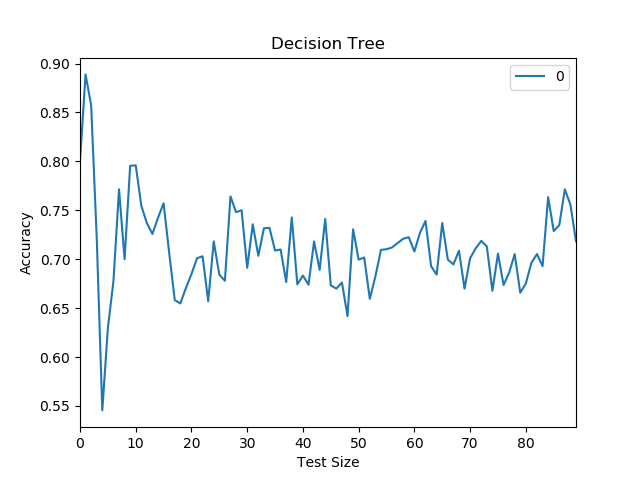
\includegraphics[scale=0.4]{dt_test_size}
	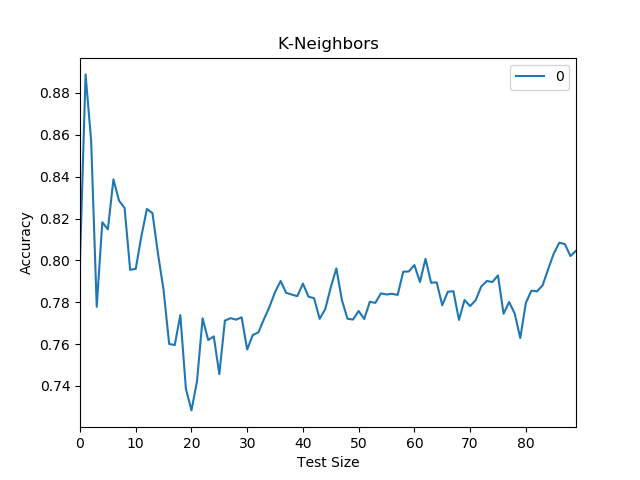
\includegraphics[scale=0.4]{kn_test_size}
	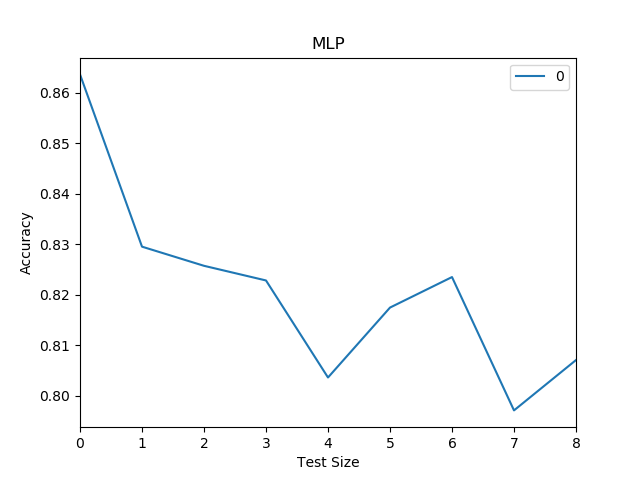
\includegraphics[scale=0.4]{mlp_test_size}
	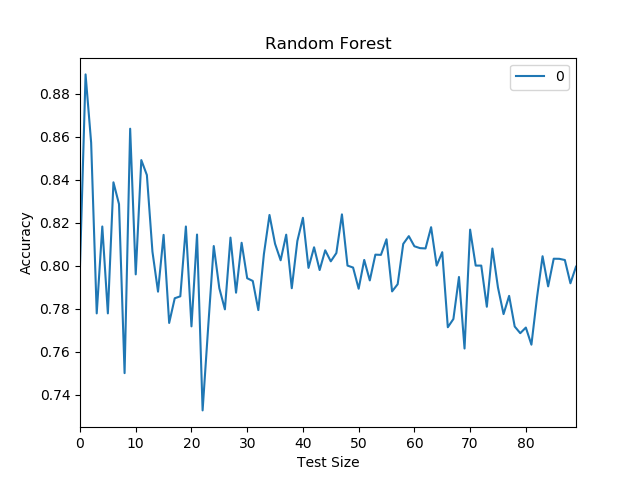
\includegraphics[scale=0.4]{rd_test_size}
  	\caption{Accuracy with different test sizes.}
  \end{center}
\end{figure}

%----------------------------------------------------------------------------------------
%	PROBLEM 2
%----------------------------------------------------------------------------------------

\section{Conclusion}
It seems that increasing the test size, or decreasing the features does not help the models to generate better outcomes. Figure 2. shows accuracy response over changing test size.
\subsection{Decision Tree}
The best one among four experiments :\textbf{ Experiment \#1.2}

In the first method (Decision Tree) results seems relatively good. Even thou in the best experiment (\#1.2) it has a good score, for \textit{True Negative} values, experiment \#1.1 was better. Best model has the third place among other models with \textbf{3} \textit{False Positive} and \textbf{2} \textit{False Negative} in total of \textbf{44} predictions.

\subsection{Random Forest}
The best one among those experiments :\textbf{ Experiment \#2.2}

It seems Decision Tree and this model both has the same accuracy value, but it can be seen from confusion matrix that \textit{True Positive/Negative} predictions are higher in this model than those predicted in Decision Tree.

On the other hand average of four experiments also higher in this method, so it is clear that Random Forest has advantages over Decision Tree.

\newpage
\subsection{ K-Nearest Neighbors}
The best one among those experiments :\textbf{ Experiment \#3.1}
It turned out this method wasn't so successful for this dataset. After many runs, it gave the lowest accuracy value every time. But it seems from experiments that this model was rather  successful about predicting \textit{True Negative} values.

\subsection{MLP Neural Network}
The best one among those experiments :\textbf{ Experiment \#4.1}
This model was the most successful one. In the experiment \#4.2 predictions was \%100 correct but even that wasn't the most successful one, the reason is unclear but experiment \#4.1 turned out to be the best.



	
\begin{figure}
 \begin{center}
	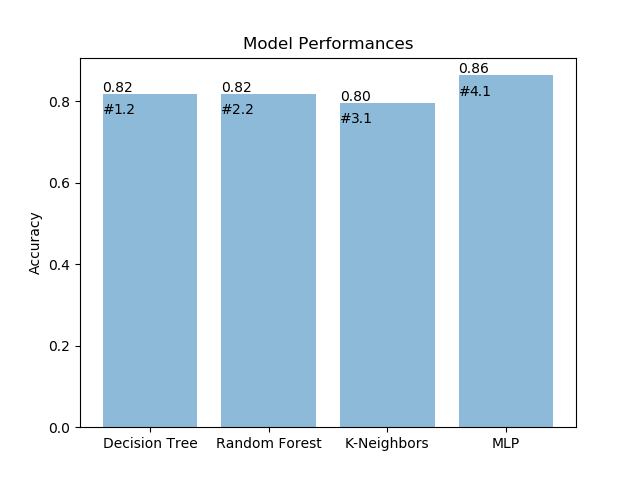
\includegraphics[scale=1]{results}
  	\caption{Model performances  }
  \end{center}
\end{figure}



\newpage
\section*{Appendix A}

Supplementary materials are located on github.com/arifbalik/DMProject

Following program runs four different models mentioned above, every model is tested with 4 different settings and best result is stored.
\begin{verbatim}
import pandas as pd
from sklearn.tree import DecisionTreeClassifier # Import Decision Tree Classifier
from sklearn.model_selection import train_test_split # Import train_test_split function
from sklearn import metrics #Import scikit-learn metrics module for accuracy calculation
from sklearn.metrics import classification_report
from sklearn.metrics import confusion_matrix
from sklearn.ensemble import RandomForestClassifier
from sklearn.neighbors import KNeighborsClassifier
from sklearn.neural_network import MLPClassifier
import matplotlib.pyplot as plt; plt.rcdefaults()
import matplotlib.pyplot as plt
import numpy as np
import warnings
warnings.filterwarnings('ignore')

pima = pd.read_csv("foreveralone.csv")

weight_m = {'Normal weight': 0, 'Underweight': 1, 'Overweight': 2, 'Obese': 3}
pima['bodyweight'] = pima['bodyweight'].map(weight_m)

income_m = {'$30,000 to $39,999': 0, '$1 to $10,000': 1, '$0': 2, '$50,000 to $74,999': 3,
'$20,000 to $29,999': 4, '$10,000 to $19,999': 5, '$75,000 to $99,999': 6,
 '$150,000 to $174,999': 7, '$125,000 to $149,999': 8, '$100,000 to $124,999': 9,
 '$174,999 to $199,999': 10, '$40,000 to $49,999': 11, '$200,000 or more':  12}
pima['income'] = pima['income'].map(income_m)

gender_m = {'Male': 0, 'Female': 1, 'Transgender male':2, 'Transgender female':3}
pima["gender"] = pima["gender"].map(gender_m)

yes_no_m = {'Yes': 1, 'No': 0}
pima["attempt_suicide"] = pima["attempt_suicide"].map(yes_no_m)
pima["depressed"] = pima["depressed"].map(yes_no_m)
pima["social_fear"] = pima["social_fear"].map(yes_no_m)
pima["virgin"] = pima["virgin"].map(yes_no_m)
pima["prostitution_legal"] = pima["prostitution_legal"].map(yes_no_m)

pay_m = {"No": 0, 'Yes': 1, "Yes but I haven't": 2}
pima["pay_for_sex"] = pima["pay_for_sex"].map(pay_m)

pima.dropna(inplace=True)



feature_cols = ['age','friends', 'depressed','social_fear', "virgin", "gender", "pay_for_sex", "income", "bodyweight"]
feature_cols2 = ['friends', 'depressed','social_fear', "virgin", "income", "bodyweight"]

y = pima.attempt_suicide

MLP = MLPClassifier(solver='adam', learning_rate='adaptive')
DT = DecisionTreeClassifier()
RF = RandomForestClassifier()
KN = KNeighborsClassifier()

performance = []
results = []
best_exp = []
for I in range(4):
    if (I == 0):
        model = DT
        print("Model: Decision Tree")
    elif (I == 1):
        model = RF
        print("Model: Random Forest")
    elif (I == 2):
        model = KN
        print("Model: K-Neighbors")
    elif (I == 3):
        model = MLP
        print("Model: MLP Neural Network")
    for K in range(4):
        if(K == 0):
            t_size = 0.1
            col = feature_cols
            X = pima[feature_cols]
        elif(K == 1):
            t_size = 0.1
            col = feature_cols2
            X = pima[feature_cols2]
        elif (K == 2):
            t_size = 0.4
            col = feature_cols
            X = pima[feature_cols]
        elif (K == 3):
            t_size = 0.4
            col = feature_cols2
            X = pima[feature_cols2]
        exp_no = (I + 1) + ((K+1) / 10)

        X_train, X_test, y_train, y_test = train_test_split(X, y, test_size=t_size, random_state=1)
        model = model.fit(X_train, y_train)
        pred = model.predict(X_test)

        print("\nExperiment #",exp_no, ", Accuracy: ", metrics.accuracy_score(y_test, pred))
        print("Test Size: ", t_size * 100 ,"%")
        print("Feature Columns: ", col)
        print(classification_report(y_test, pred))
        print("Confusion Matrix:\n", confusion_matrix(y_test, pred))
        results.append(metrics.accuracy_score(y_test, pred))

    performance.append(max(results))
    best_exp.append((I + 1) + (results.index(max(results)) +1)/10)
    print("\nBest Experiment: #",best_exp[I],", Accuracy: ", max(results))
    del results[:]


objects = ( 'Decision Tree', 'Random Forest', 'K-Neighbors', 'MLP')
y_pos = np.arange(len(objects))

bars = plt.bar(y_pos, performance, align='center', alpha=0.5)
plt.xticks(y_pos, objects)
ix = 0
for bar in bars:
    yval = bar.get_height()
    plt.text(bar.get_x(), yval - .05, '#')
    plt.text(bar.get_x() + 0.09, yval - .05, best_exp[ix])
    plt.text(bar.get_x(), yval + .005, '%.2f' % yval)
    ix = ix + 1
plt.ylabel('Accuracy')
plt.title('Model Performances')
plt.show()

\end{verbatim}

\newpage
\section*{Appendix B}

Following figures shows tree diagrams of the Decision Tree algorithm

\end{document}
